\newpage
\section{Evalutaion einer symmetrischen Antenne}
Das Abstrahlverhalten von Loop und Dipol Antennen ist im Fernfeld gleich. Im Fernfeld steht das E und das
H Feld senkrecht aufeinander. Senkrecht zum E und H Feld zeigt sich der Ausbreitungsvektor. Die elektrischen und
magnetischen Feldkomponenten sind in Phase. Daher wird im Fernfeld Wirkleistung in transversale Raumrichtung
übertragen. Das elektrische und magnetische Feld hat nur Komponenten in der Ebene senkrecht zur Ausbreitungsrichtung.
Man spricht von einer ebenen Welle. Sie wird vom E und H Vektor aufgespannt  und bewegt sich in
Transversalerrichtung fort. Die Kugelwelle bewegt sich im Raum fort, bis die gesamte Energie absorbiert ist. Die Amplituden der E und H Vektoren
nehmen mit steigendem Abstand r um den Faktor $1/r$  ab. Der Zusammenhang zwischen E und H Feld ist
durch die intrinsische Wellenimpedanz $\eta$ gegeben. 
Die Gleichung \ref{eq:WellenImpedanzZ0} zeigt den Wellenwiderstand im Vakuum.

\begin{equation}\label{eq:WellenImpedanzZ0}
Z_{0}=\dfrac{E}{H}=\sqrt{\dfrac{\mu}{\epsilon}}=377\Omega
\end{equation}



Die Ausrichtung des E Feldes ist bei den Loop und den Dipol Antennen um 90 Grad verschoben. 
Im Nahfeld sind die induktiven Anteile des elektromagnetischen Wechselfeldes bei den Loop Antennen dominant. 
Im Gegenzug ist das Nahfeld der Dipol Antenne mehr kapazitiv.
Mann nennt die Dipolantenne deshalb E Feld Antenne und die Loop Antenne wird oft H Feld Antenne genannt.
Das Abstrahlverhalten ist in den Kapitelen \ref{sec:DipolAntenne} und \ref{sec:LoopAntenneTheorie} aufgezeigt. Die Abbildung \ref{fig:FerdVektorEinheistsvektor} zeigt einen Pointingvektor im  kugelkoordinaten und im kartesischen Koordinatensystem. Am Ende des Pointingvektor $\vec{r}$  sind die Einheitsvektoren mit den dazugehörenden  E und H Feldvektoren ersichtlich.\\

%%%%%%%%%%%%%%%%%%%%%%%%%%%%%%%%%%%
\begin{figure}[h]
\begin{center}
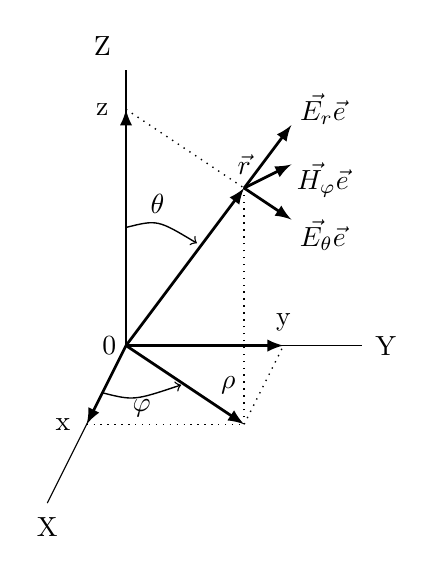
\begin{tikzpicture}
	\draw (4,4) -- (3,2)node at (3, 1.7) {X};%Fadenkreuz x
	\draw (4,4) node[left] {0} -- (7,4)node at (7.3, 4) {Y};%Fadenkreuz y
	\draw (4,4) -- (4,7.5)node at (3.7, 7.8) {Z};%Fadenkreuz z
	
	\draw[line width=1pt, ->, >=latex](4, 4)  -- (3.5, 3) node at (3.2, 3) {x};
	\draw[line width=1pt, ->, >=latex](4, 4)  -- (6, 4) node at (6, 4.3) {y};
	\draw[line width=1pt, ->, >=latex](4, 4)  -- (4, 7) node at (3.7, 7) {z};
	
	\draw[line width=0.5pt, style=dotted](3.5, 3) -- (5.5, 3);%Projektion y Rcihtung
	\draw[line width=0.5pt, style=dotted](5.5, 3) -- (6, 4);%Projektion x Rcihtung
	
	\draw[line width=1pt, ->, >=latex](4, 4)  -- (5.5, 3) node at (5.3, 3.5) {$\rho$};
	
	\draw[line width=1pt, ->, >=latex](4, 4)  -- (5.5, 6) node at (5.5, 6.3) {$\vec{r}$};
	
	\draw[line width=0.5pt, style=dotted](5.5, 3) -- (5.5, 6);%Projektion p zu \vec{r}
	\draw[line width=0.5pt, style=dotted](4, 7) -- (5.5, 6);%Projektion von z zur \vec{r}
	
	\coordinate (A) at (4, 5.5);
	\coordinate (B) at (4.9, 5.3);
	\coordinate (a) at (4.4, 5.6);
	\draw[line width=0.5pt, cap=round,->](A) .. controls (a) .. (B) node at (4.4, 5.8){$\theta$};
	
	\coordinate (C) at (3.7, 3.4);
	\coordinate (D) at (4.7, 3.5);
	\coordinate (c) at (4.1, 3.3);
	\draw[line width=0.5pt, cap=round,->](C) .. controls (c) .. (D) node at (4.2, 3.2){$\varphi$};
	
	%Einheitsvektoren
	\draw[line width=1pt, ->, >=latex](5.5, 6)  -- (6.1, 6.8) node at (6.5, 7) {$\vec{E_{r}}\vec{e}$};
	\draw[line width=1pt, ->, >=latex](5.5, 6)  -- (6.1, 5.6) node at (6.5, 5.4) {$\vec{E_{\theta}}\vec{e}$};
	\draw[line width=1pt, ->, >=latex](5.5, 6)  -- (6.1, 6.3) node at (6.5, 6.1) {$\vec{H_{\varphi}}  \vec{e}$};
	
\end{tikzpicture}
\end{center}
	\caption{Feldvektor mit Einheitsvektoren}
	\label{fig:FerdVektorEinheistsvektor}
\end{figure}

Die Oberfläche  der elektromagnetischen Welle nimmt mit steigendem Abstand r von der Antenne immer weiter zu. Ebenfalls nimmt die Beugung der Oberfläche der Kugelwelle immer mehr ab. Ist der Abstand r genügend gross, so kann die Welle lokal als ebene Wellenfront angenommen werden. Bei Distanzen von mehr als $2\lambda$ kann das Fernfeld angenommen werden, es gilt das Fernfeldkriterium. Bei einer Zielfrequenz von 2.45 Ghz bei der die Bluetooth Antenne arbeiten soll, tritt das Fernfeld wie in der Gleichung \ref{eq:Fernfeld} gezeigt nach 24 cm auf.



\begin{align}\label{eq:Fernfeld}
\lambda &=\dfrac{c}{f} \\
\lambda &=\dfrac{3E8[m/s]}{2.45E9[1/s]}=0.12m\\ \nonumber
2\lambda &= Fernfeldkriterium\\ \nonumber
2\lambda &= 2*0.12[m] =0.24[m] \nonumber
\end{align}

Es kann kein eindeutiger Betriebsfall für die "Connect 1"\  Geräte genannt werden. Es ist wahrscheinlich, dass die meisten der Tuchfliegerpiloten die "Connect 1"\  Geräte zur Navigation verwenden. Das Gerät wird auf dem Schoss getragen. Dabei wird das Gerät in einer Hülle mit Bändern am Oberschäkel befestigt. Ein Mobiltelefon, welches sich am Arm des Piloten oder in einer Brusttasche befindet, ist klar mehr als $2\lambda$ entfernt und somit im Fernfeld. Da sowohl die Loop als auch die Dipol Antenne ein Torus ähnliches Fernfeld aufzeigen und die Position der neuen Bluetooth Antenne für beide Antennen die selbe sein wird, sind die Nahfeldeigenschaften der Antennen von Bedeutung.

\subsection{Eigenschaften der Antenne}\label{sec:EigenschaftenAntenne}
Die 2.4 GHz Bluetooth Antenne wird im Gerät "Connect 1" der Flytec eingesetzt. Dies ist ein kompaktes Handgerät welches den Piloten eines Tuchfliegers bei der Navigation in der Luft unterstützt. Die Gerätabmessungen sind 142 x 88 x 23 mm (L x B x H). Der Raum der die neue Antenne einnehmen wird ist nicht derselbe wie in der Vorgängerversion der "Connect 1" \ Hardware. Für die neue Positionierung der Antenne wird der Hohlraum zwischen der Seitenwand des ABS Kunsstoffgehäuses und der Hauptplatine  vorgesehen. Das mögliche Antennenvolumen beschränkt sich somit auf 55 x 10 x 3.5 mm (L x B x H).\\
Die Speisung der neuen Bluetooth Antenne soll nicht wie bis anhin asymmetrisch sein. Wie der Antennenfusspunkt mit der Quelle verbunden wird ist zum jetzigen Zeitpunkt noch nicht definiert. Mögliche symmetrische Verbindungen sind:

\begin{itemize}
\item Microstrip Verbindung  
\item Zweidrahtleitung
\item Zweidrahtleitung in Form eines Koaxialkabels
\end{itemize}

Die symmetrische Verbindung zwischen Quelle und Antenne hat den Vorteil, dass die bis anhin verwendeten Baluns für die Umwandlung des symmetrischen Ausgangs des Transsivers nicht mehr benötigt werden. \\
Die Ausgangsimpedanz des verwendeten Texas Instruments CC2541 Transsivers ist bei 2.440 GHz $(70+j30) Ohm$. Dies entspricht einer komplexen Ausgangsimpedanz. \\Bei den gemachten Aussagen zu den Simulationen wurde jedoch eine rein reele Quellimpedanz von $(50+j0) Ohm$ angenommen.

\subsection{Dipol Antenne}
Die Dipol Antenne ist eine häufig vorkommende Antennenform.  Wird der Halbwellendipol mit seiner Resonanzfrequenz $f=\dfrac{\lambda}{2}$ angesteuert, tritt ein maximales Schwingen des Dipols auf.
%%%%%%%%%%%%%%%%%%%%%%%%%%%%%%%%%%%%%%%%%%%%%%%%%%%
\begin{figure}[h]%ESB Antenne
	\begin{center}
	\begin{tikzpicture}
	\draw[line width=1.5pt](5, 2) circle (0.5) node at (5, 2) {AC};
	\draw[line width=1pt, -*](4.8, 2.45) -- (4.8, 3.6);%nach oben links
	\draw[line width=1pt, -*](5.2, 2.45) -- (5.2, 3.6);%nach oben rechts
	
	\draw[line width=3pt](4.8, 3.5) -- (2, 3.5);%links
	\draw[line width=3pt](5.2, 3.5) -- (8, 3.5);%rechts
	
	\draw[line width=1pt, ->, >=latex](3.8, 3.7)  -- (3, 3.7) node at (3.4, 3.9) {I};%Strompfeil links
	\draw[line width=1pt, ->, >=latex](6.2, 3.7)  -- (7, 3.7) node at (6.6, 3.9) {I};%Strompfeil rechts	
	
	\coordinate (A) at (2, 3.5);%Bogen
	\coordinate (B) at (8, 3.5);
	\coordinate (a) at (5, 5.2);
	\draw[line width=1pt, cap=round](A) .. controls (a) .. (B);
	
	\draw[line width=0.5pt, style=densely dashed](1.8, 3.5) -- (1.8, 5.5);%nach oben links
	\draw[line width=0.5pt, style=densely dashed](8.2, 3.5) -- (8.2, 5.5);%nach oben rechts
	\draw[line width=0.5pt, style=densely dashed](1.7, 5.4) -- (8.3, 5.4) node at (5, 5.7) {$\lambda/2$};%langer Strich
	
	\end{tikzpicture}
	\end{center}
\caption{horizontalpolarisierter Halbwellendipol}
\label{fig:HalbWellenDipolHorizontal}
\end{figure}
%%%%%%%%%%%%%%%%%%%%%%%%%%%%%%%%%%%%%%%%%%%%%%%%%%%%%%%%%%%%


Gegenüber idealen Betrachtungen muss die Länge des $\lambda /2$ Dipols um den Faktor 0,95 kürzer gewählt werden, um  die gewünschte Frequenz zu erhalten. Die Verkürzung  ist in der Abbildung \ref{fig:HalbWellenDipolHorizontal} gezeigt.

%Weiter Komentar wiso es sich eine Verkürtzung einstellt
%H. Cuno, Vorbereitung auf die Amateurfunklizenzprüfung, Frech-VerlagStuttgart, 1976 
Ideale Betrachtungen gehen von einem unendlich dünnen Draht aus, wobei der Dipol im
ungestörten Raum betrieben wird. Aufgrund der geforderten mechanischen Festigkeit
müssen reale Dipole eine gewisse Mindestdicke aufweisen. Die Umgebung des Dipols kann
ebenfalls nicht als völlig freier Raum angenommen werden. Es befindet sich immer eine Quelle oder eine Zuleitung oder beides in der Nähe von realen Antennen. Die Dipolenden weisen eine höhere Kapazität als im Idealzustand auf und die Resonanzfrequenz sinkt. 
%ist das richtig?

Wenn sich eine $\lambda /2$ lange Vertikalantenne über der Erde befindet,  ergeben sich für das Strahlungsdiagramm die folgenden Eigenschaften: 
Die Horizontalcharakteristik des vertikalen Halbwellendipols ist kreisförmig aufgrund der Symmetrie. Das Strahlungsdiagramm ist unabhängig vom Azimutwinkel $\varphi$ in der Horizontalebene des Dipols. Die Vertikalcharakteristik des vertikalen Halbwellendipols über der Erde erscheint jedoch gerichtet, das heisst es besteht eine Abhängigkeit vom Winkel $\theta$ . 

Gemäss O. Zinke %O. Zinke, H. Brunswig, Lehrbuch der Hochfrequenztechnik, Band 1, 4. Auflage,Springer-Verlag, Berlin Heidelberg New York, 1990
 lassen sich die folgenden Aussagen für einen Dipol vertikal Polarisiert über der Erde treffen:


\begin{equation}\label{eq:FDipolTheat}
F(\theta,\frac{l}{\lambda}=\dfrac{1}{2})=\dfrac{2\cos^{2}(\dfrac{\pi}{2}\cos\theta)}{\sin\theta}
\end{equation}

%Braut es eventuell noch ein Bild

Die Nahfeldeigenschaften der Dipol Antenne zeigt ein starkes E Feld. Dieses zeigt eine Richtungsabhängigkeit  des Winkels $\theta$. Die starken E Felder polarisieren alle Dielektrika in unmittelbarer Nähe des Dipols. Dies führt zu dielektrischen Verlusten. Diese steigen mit der Frequenz des Feldes. Die dielektrischen Verluste können als Widerstände in Serie gedacht werden. Sie stellen die äquivalente Verlustleistung an einem Widerstand dar, die für das polarisieren der umgebenden dielektrikum Struktur nötig ist.
Das Dielektrikum ist ein elektrisch nicht leitendes Material, das aber vom elektrischen Feld durchdringt wird. Die Feldgrössen des Dielektrikums sind die elektrische Feldstärke E und die elektrische Flussdichte D. Die Flussdichte D ist  im elektrostatischen Fall, das heisst im zeitlich konstanten Fall, und in einem isotropen Medium durch die Primitivität $\varepsilon $ \ über folgende Beziehung in Gleichung \ref{eq:FlussdichteD} verknüpft:



\begin{equation}\label{eq:FlussdichteD}
D=\varepsilon E
\end{equation}

Die Permittivität $\varepsilon$ setzt sich, wie in Gleichung \ \ref{eq:Epsilon} ersichtlich, aus der elektrischen Feldkonstante $\varepsilon_0$ und der materialspezifischen, relativen Permittivität $\varepsilon_r$ zusammen:
\begin{equation}\label{eq:Epsilon}
\varepsilon = \varepsilon_r \varepsilon_0
\end{equation}

Da in einem Dielektrikum die Ladungsträger nicht frei beweglich sind, werden sie durch ein äusseres elektrisches Feld polarisiert. Dabei wird zwischen zwei Arten der Polarisation unterschieden:
\begin{itemize}
\item Verschiebungspolarisation
\item Orientierungspolarisation
\end{itemize}

Bei der Verschiebungspolarisation werden elektrische Dipole  induziert. Das heisst,  die Dipole entstehen durch geringe Ladungsverschiebung in den Atomen, Molekülen oder zwischen verschieden geladenen Ionen. Bei einem Wechselfeld schwingt die negative Elektronenhülle und der positive Atomkern gegenläufig hin und her.  Bei diesen Schwingungen entsteht  Wärmeenergie.  Diese kann gegenüber der Energie, die bei der Orientierungspolarisation ensteht,  vernachlässigt werden.  Die Bewegung des Atomkerns kann auf Grund seiner deutlich grösseren Masse  gegenüber der Elektronenhüllenbewegung vernachlässigt werden. Somit wird der Atomkern als ortsfest betrachtet. 

Unter der Orientierungspolarisation versteht man die Ausrichtung ungeordneter, permanenter Dipole eines Isolators im elektrischen Feld. Bei einem Wechselfeld müssen sich die Moleküle ständig umorientieren, wodurch Wärmeenergie entsteht.

Im Nahfeld einer Antenne pendelt die nicht abgestrahlte Energie im Raum um die Antenne hin und her. Das Nahfeld baut sich auf und ab. Es wechselt so mit der Resonanzfrequenz $f_r$ seine Richtung. Die Moleküle im dielektrischen Raum um die Antenne werden bei jeder Schwingung neu polarisiert.
Die im Dielektrikum gespeicherte Energie ist stark von der materialspezifischen, relativen Permittivität $\varepsilon_r $ abhängig. 

Die dielektrischen Verluste führen bei Antennen auch zu einem Detuning. Das Detuning ist kaum zu berechnen, aber es kann mit Simulationen bestimmt werden. Das Detuning entsteht durch Verluste in und um die  Antenne, da die komplexe Impedanz der Antenne verändert wird. Das Detuning kann auch eine Chance darstellen. Es ist denkbar, dass durch das Detuning und die veränderte Antennenimpedanz eine Anpassung an den Sender und die Zuleitung entsteht und so eine wesentlich höhere Abstrahleffizienz $\eta_{overall}$ \ sich ergibt.

Im Zusammenhang der Antennen und den reaktiven Nahfeldverlusten wird oft der Verlustwinkel genannt.  Der Verlustwinkel beschreibt den Anteil der Wirkleistung elektrisch reaktiver Bauteile wie Spulen oder Kondensatoren bei sinusförmigen Spannungs- und Stromverlauf. 

Der Verlustwinkel ist als $\arctan$ des Verhältnisses von Wirkleistung zu Blindleistung definiert. 
Je kleiner der Verlustwinkel, desto näher kommen die realen Bauteile ihrem idealen Verhalten. Eine ideale Induktivität hat einen Verlustwinkel von $0^\circ$. Ein idealer Kondensator hat ebenfalls einen Verlustwinkel von 0$^\circ$. Ein Verlustwinkel der grösser ist als $0^\circ$ führt zu Verlustwiderständen die in Serie zu den idealen Induktivitäten und Kapazitäten gerechte werden.

Ein idealer elektrischer Widerstand hat dagegen einen Verlustwinkel von $90^\circ$. Er besitzt keine kapazitiven oder induktiven Blindanteile.

In der technisch realisierbaren Elektronik gibt es aber keine idealen Bauteile. Die Verluste sind zudem frequenzabhängig.

Der Verlustwinkel  $\delta$  lässt sich über die komplexe Impedanz Z oder über die Phasenverschiebung  $\varphi$  zwischen Strom und Spannung des Bauteils berechnen: 

\label{eq:Verlustwinkel}
\begin{align}
\delta &= \arctan \dfrac{Re\underline{Z}}{Im\underline{Z}} \\
\delta &= 90^\circ - |\varphi|
\end{align}

Die realen Ersatzschaltbilder von Spulen und Kondensatoren berücksichtigen die Verluste mit einem R.
Die beiden Gleichungen \ref{eq:VerlustwinkelSpule} und \ref{eq:VerlustwinkelKondensator} zeigen die Verlustfaktoren an einer Spule und an einem Kondensator:

\begin{equation}\label{eq:VerlustwinkelSpule}
\tan \delta = \dfrac{R}{\omega L}
\end{equation}

\begin{equation} \label{eq:VerlustwinkelKondensator}
\tan \delta = R \omega C
\end{equation}

In diesem Zusammenhang soll auch die komplexe Permittivität $\varepsilon$ genannt werden:
\begin{equation} \label{eq:komplexePermitivität}
\varepsilon=\varepsilon_0(\varepsilon^{'}-j\varepsilon^{''})=\varepsilon_0\varepsilon^{'}(1-j\dfrac{\varepsilon^{''}}{\varepsilon^{'}})
\end{equation}

In der Gleichung \ref{eq:komplexePermitivität} kommt das Verhältnis $\dfrac{\varepsilon^{''}}{\varepsilon^{'}}$ vor. Das Verhältnis ist klein für gute Dielektrika, welche über einen weiten Frequenzbereich annähernd konstant sind. Das Verhältnis von der Wechselstrom Permittivität $\varepsilon^{'}$ und des dielektrischen Verlustfaktor $\varepsilon^{''}$ ergibt den Verlustwinkel $\tan\delta$

\begin{equation} \label{eq:VerlustwinkelEpsilonPermitivität}
\dfrac{\varepsilon^{''}}{\varepsilon^{'}}=\tan\delta
\end{equation}


\subsubsection{Verwendung einer Dipolantenne im Connect 1}
Eine symmetrisch gespiesene Halbwellenantenne die leicht verkürzt ist,  ist eine einfach zu produzierende Antenne. Halbe Wellenlänge als strahlende Leiterlänge bedeutet etwas weniger als 0.06m Strahlerlänge. Das ist in dem Schlitz zwischen der Hauptplatine und der Gehäuseaussenelementen unterzubringen. 
Das bedeutet, das die Antenne von sehr viel ABS Kunststoffmaterial umgeben ist. Dieses Material ist elektrisch nicht leitend und nicht magnetisch. Alle Dipolantennen sind in ihrem unmittelbaren Umfeld starke E Feld Strahler.  Die Materialeigenschaften von ABS Kunststoff führen mit einem  $\varepsilon_r$ von ca. 4.2 bei 2.4 GHz zu einer erheblichen Energiespeicherung im reaktiven Nahfeld der Antenne. Das führt wiederum zu einer Abweichung der idealen Antennenimpedanz. Die Veränderung der Antennenimpedanz bringt wiederum ein Detuning der Antenne mit sich.

Ein Beispiel einer Dipolantenne mit und ohne ABS Kunststoff im Nahfeld.

Das Abstrahlverhalten ist $\theta$ abhängig. Die Richtkarakteristik oder auf englisch directivity D genannt, ist bei Dipolantennen wie in Formel \ref{eq:Directivity} gezeigt 1.64dBi. Die directivity vergleicht die Leistungsdichte in der stärksten Abstrahlrichtung, mit der Leistungsdichte eines isotropen Kugelstralers bei gleicher totaler abgestrahlter Leistung. 

Der Strahlungswiderstad des $\lambda/2$ Dipols enspricht wie in Gleichung \ref{RradDipol} 73 Ohm. Dies ist ein theoretischer Wert, bei technisch realisierbaren Halbwellendipolen wird der Strahlungswiderstand $R_{rad}$ kleiner als 70 Ohm. Zudem kommt  ein von der  geometrie der Antenne abhänige reaktanz $X_{ant}$ hinzu.
Die Reaktanz $X_{ant}$ und der Strahlungswiderstand $R_{rad}$, sowie der Verlustwiderstand $R_v$ ergeben die Antennenimpedanz, diese wird $Z_{ant}$  genannt. Dieser Zusammenhang ist  in der Abbildung \ref{fig:ESBantenneZant} gezeigt.

%%%%%%%%%%%%%%%%%%%%%%%%%%%%%%%%%%%%%%%%%%%%%%%%%%%
\begin{figure}[h!]%ESB Antenne mit Zant
	\begin{center}
	\begin{tikzpicture}
%	\draw[line width=1.5pt](7, 1.5) rectangle (12, 5.5) node at (9.5, 6) {Anpassungsnetzwerk};
	\draw[line width=1.5pt, *-](12, 5)  -- (13.5, 5);
	\draw[line width=1.5pt, *-](12, 2)  -- (16, 2);
	\draw[line width=1.5pt](13.5, 4.75) rectangle (14.5, 5.25) node at (14, 5.5) {$R_{v}$};
	\draw[line width=1.5pt](14.5, 5)  -- (16, 5);
	\draw[line width=1.5pt](16, 5)  -- (16, 4.4);
	\draw[line width=1.5pt](15.75, 3.4) rectangle (16.25, 4.4) node at (17, 3.9) {$R_{rad}$};%Rrad
	\draw[line width=1.5pt](16, 3.4)  -- (16, 2.8);
	\draw[line width=1.5pt](15.75, 2.8)  -- (16.25, 2.8);%Kondensator oben
	\draw[line width=1.5pt](15.75, 2.6)  -- (16.25, 2.6);%Kondensator unten
	\node at (17, 2.7) {$X_{ant}$};
	\draw[line width=1.5pt](16, 2.6)  -- (16, 2);
	
%	\draw[line width=1.5pt, ->, >=latex](6.5, 4)  -- (8, 4) node at (8, 3.5) {$P_{ein}$};
%	\draw[line width=1.5pt, ->, >=latex](11.5, 4)  -- (13, 4) node at (13, 3.5) {$P_{ant}$};
	

%	\draw [-latex,line width=1.5pt](11.5,1) |-(13,2.5) node at (11.5, 0.5) {$Z_{ant}$};
	
%	\node at (17.5, 6) {$\eta_{rad}=\dfrac{R_{rad}}{Rv+R_{rad}}$};
%	\node at (9.5, 7) {$\eta_{overall}=\dfrac{P_{rad}}{P_{ein}}$};
	
%	\node at (18, 2.7) {$\varepsilon$};
%	\node at (18.5, 2.7) {$\delta$};
	
	\draw[->,line width=0.5pt,decorate, decoration=snake ](18, 4.1) -- (19.5, 4.6);
	\draw[->,line width=0.5pt, decorate, decoration=snake](18, 3.9) -- (19.5, 3.9);
	\draw[->,line width=0.5pt, decorate, decoration=snake](18, 3.7) -- (19.5, 3.1);
	\node at (20, 3.9) {$P_{rad}$};
	
	\draw[line width=1.5pt, decorate, decoration=brace] (13, 1) -- (16.5, 1) node at (14.75, 0.5) {$Z_{ant} =  R_v + R_{rad} + X_{ant}$};
	\end{tikzpicture}
	\end{center}
\caption{Ersatzschaltbild einer Antenne mit $Z_{ant}$}
\label{fig:ESBantenneZant}
\end{figure}
%%%%%%%%%%%%%%%%%%%%%%%%%%%%%%%%%%%%%%%%%%%%%%%%%%%%%%%%%%%%








\subsubsection{Halbwellen Dipol Eigenschaften}
Das Ersatzschaltbild in der Abbildung \ref{fig:ESBantenne} einer Antenne zeigt die wesentlichen Parameter, die für eine Beurteilung der Abstrahleffizienz verantwortlich sind. Es sind dies:
\begin{itemize}
\item $R_{v}$
\item $R_{rad}$
\item $Z_{ant}$
\end{itemize}

Weitere wichtige Eigenschaften, die für die Auswahl eines Antennentyps in die Geräte der "Connecte 1" \  Serie zu berücksichtigen  sind:
\begin{itemize}
\item Directivity D
\item Nahfeldtyp
\item Detuning durch das Umgebungsmaterial
\item Kopplung mit anderen im Gerät vorhandenen Antennen
\end{itemize}

%%%%%%%%%%%%%%%%%%%%%%%%%%%%%%%%%%%%%%%%%%%%%%%%%%%
\begin{figure}[h]%ESB Antenne
	\begin{center}
	\begin{tikzpicture}
%	\draw[line width=1.5pt](7, 1.5) rectangle (12, 5.5) node at (9.5, 6) {Anpassungsnetzwerk};
	\draw[line width=1.5pt, *-](12, 5)  -- (13.5, 5);
	\draw[line width=1.5pt, *-](12, 2)  -- (16, 2);
	\draw[line width=1.5pt](13.5, 4.75) rectangle (14.5, 5.25) node at (14, 5.5) {$R_{v}$};
	\draw[line width=1.5pt](14.5, 5)  -- (16, 5);
	\draw[line width=1.5pt](16, 5)  -- (16, 4.4);
	\draw[line width=1.5pt](15.75, 3.4) rectangle (16.25, 4.4) node at (17, 3.9) {$R_{rad}$};%Rrad
	\draw[line width=1.5pt](16, 3.4)  -- (16, 2.8);
	\draw[line width=1.5pt](15.75, 2.8)  -- (16.25, 2.8);%Kondensator oben
	\draw[line width=1.5pt](15.75, 2.6)  -- (16.25, 2.6);%Kondensator unten
	\node at (17, 2.7) {$X_{ant}$};
	\draw[line width=1.5pt](16, 2.6)  -- (16, 2);
	
%	\draw[line width=1.5pt, ->, >=latex](6.5, 4)  -- (8, 4) node at (8, 3.5) {$P_{ein}$};
	\draw[line width=1.5pt, ->, >=latex](11.5, 4)  -- (13, 4) node at (13, 3.5) {$P_{ant}$};
	

	\draw [-latex,line width=1.5pt](11.5,1) |-(13,2.5) node at (11.5, 0.5) {$Z_{ant}$};
	
	\node at (17.5, 6) {$\eta_{rad}=\dfrac{R_{rad}}{Rv+R_{rad}}$};
%	\node at (9.5, 7) {$\eta_{overall}=\dfrac{P_{rad}}{P_{ein}}$};
	
	\node at (18, 2.7) {$\varepsilon$};
	\node at (18.5, 2.7) {$\delta$};
	
	\draw[->,line width=0.5pt,decorate, decoration=snake ](18, 4.1) -- (19.5, 4.6);
	\draw[->,line width=0.5pt, decorate, decoration=snake](18, 3.9) -- (19.5, 3.9);
	\draw[->,line width=0.5pt, decorate, decoration=snake](18, 3.7) -- (19.5, 3.1);
	\node at (20, 3.9) {$P_{rad}$};
	\end{tikzpicture}
	\end{center}
\caption{Ersatzschaltbild einer Antenne}
\label{fig:ESBantenne}
\end{figure}
%%%%%%%%%%%%%%%%%%%%%%%%%%%%%%%%%%%%%%%%%%%%%%%%%%%%%%%%%%%%

Der $R_{v}$ vereint die elektrischen Verluste, die in den Leitern und an den Übergängen zu stande kommen. Ebenfals kann der $R_{rad}$ nicht einfach ausgemessen werden, $R_{rad}$ entspricht dem Widerstand der benötigt wird, um beim frequenzabhängig resultierenden Antennenstrom die abgestrahlte Leistung umzuwandeln.\\
Das Verhältnis von $R_{rad}$  zu $R_{v}$ wirkt direkt in die Abstrahleffizienz $\eta_{rad}$. \\
Die Antennenimpedanz ist in der Abbildung \ref{fig:ESBantenne} als $X_{ant}$ in Form eines Kondensators abgebildet. Die Dielektrischenverluste des Winkels $\delta$ wirken ebenfals in den $R_{v}$.\\
Die drei Komponenten $R_{v}$, $R_{rad}$ und $X_{ant}$ ergeben zusammen die gesammte Antennenimpedanz $Z_{ant}$.


Der Strahlungswiderstand $R_{rad}$ des Halbwellen Dipols wird in der Gleichung \ref{eq:Rrrad} im Kapitel \ref{sec:kurzerDipol} berechnet. Man erhält für einen Dipol mit $2L = \frac{\lambda}{2}$ einen $R_{rad}$ von $15.7 \Omega $.

\newpage
\subsubsection{Simulationen eines Halbwellen Dipol}

Das Volumen in dem eine Bluetooth Antenne untergebracht werden kann ist in Kapitel \ref{sec:EigenschaftenAntenne} beschrieben. Das Volumen von 55 x 10 x 3.5 mm (L x B x H) wurde bei den Simmulationen berücksichtigt. \\
Für die Simmulationen wurden grosse Vereinfachungen getroffen.\\
Der ABS Kunststoff ist mit einem $\varepsilon_r $ von 4.3 und einem Verlustwinkel von 0.02 simuliert. Als Antennenstäbe wurde ein  Kupferdraht mit einem Radius $r = 1.12 mm$ verwendet. Das Kupfer hat eine Leitfähigkeit von $\kappa=58E6 [1/\Omega m]$. Die Länge der beiden Antennenarme ist je 25mm. Für die Quelle wurde eine Lücke von 2.45mm ausgespart. Die Quelle ist als 50 Ohm reel definiert.\\ 
Es wurden drei Simulationen durchgeführt.
\begin{enumerate}
\item  $\lambda/2 \ $Dipol im Freiraum
\item  $\lambda/2 \ $Dipol mit angrenzendem ABS Stück
\item  $\lambda/2 \ $Dipol eingklemmt zwischen zwei ABS Stücken
\end{enumerate}

Die Abbildung \ref{fig:S11_Dipol_freiraum_1} zeigt das $S_{11}$ Diagramm eines Dipols im Freiraum. Die Resonanzfrequenz ist bei 2.42 GHz abgestimmt und es resuliert eine Return Loss Dämpfung von -16.1dB. Die 3dB Bandbreite ist etwa 200MHz und liegt bei ca. -13.1dB. Das zu dieser Freiraum Simulation gehöhrende Smith Diagramm zeigt in der Abbildung \ref{fig:Smith_Dipol_freiraum_2}  bei der Resonazfrequenz einen Widerstand von 68.6 Ohm reel. Das ist nahe dem in der Theorie und mit der Formel \ref{RradDipol} gezeigten Wert von 73 Ohm. Das Smith Diagramm zeigt weiter einen kapazitiven  Imaginäranteil von $j-4\Omega$. Da die Anpassung an die Quellenimpedanz von reel 50 Ohm gut stimmt, wird eine hohe Abstrahleffizienz von $\eta = 97.5 \% $ erreicht.
\begin{figure}[!h]
\begin{center}
\minipage{0.4\textwidth}
  \includegraphics[width=\linewidth]{content/bilder/Evaluation/Dipol/S11DipolOhneABS.pdf}
  \caption{\\S11 Diagramm \\eines Dipols in Freiraum}\label{fig:S11_Dipol_freiraum_1}
\endminipage%\hfill
\minipage{0.32\textwidth}
  \includegraphics[width=\linewidth]{content/bilder/Evaluation/Dipol/SmithDipolOhneABS.pdf}
  \caption{\\Smith Diagramm eines Dipols im Freiraum}\label{fig:Smith_Dipol_freiraum_2}
\endminipage
\end{center}
\end{figure}

In der Abbildung \ref{fig:S11_Dipol_ABS_3} wird das $S_{11}$ Diagramm eines Dipols mit einem ABS Kuststoffstück im Nahfeld gezeigt. Das ABS Stück hat die Masse: 100 x 30 x 2 mm (L x B x H). Es ist direkt an die Antennenstäbe angrenzend. Die dielektrischen Verluste zeigen sich im Detuning der Resonazfrequenz in der Abbildung \ref{fig:S11_Dipol_ABS_3}. Der maximale $S_{11}$ Wert liegt neu 400 MHz tiefer bei 2.04 GHz. Der $S_{11}$ Wert bei dieser Frequenz beträgt  neu -20.79dB.\\
Das Smith Diagramm in Abbildung \ref{fig:Smith_Dipol_ABS_4} zeigt die Fehlanpassung. Bei der Wunschfrequenz von 2.45 GHz entspricht der Realteil der Antennenimpedanz 141 Ohm und der Imaginärteil ist mit $j+39$ Ohm induktiv.
\begin{figure}[!h]
\begin{center}
\minipage{0.4\textwidth}
  \includegraphics[width=\linewidth]{content/bilder/Evaluation/Dipol/S11DipolABS.pdf}
  \caption{\\S11 eines Dipols mit \\angrenzendem ABS Stück}\label{fig:S11_Dipol_ABS_3}
\endminipage%\hfill
\minipage{0.32\textwidth}
  \includegraphics[width=\linewidth]{content/bilder/Evaluation/Dipol/SmithDipolABS.pdf}
  \caption{\\Smith Diagramm eines Dipols mit angrenzendem ABS Stück}\label{fig:Smith_Dipol_ABS_4}
\endminipage
\end{center}
\end{figure}

\newpage
Die drite Simulation zeigt, das $S_{11}$ und das Smith Diagramm der Antenne, die zwischen zwei ABS Kunststoffstücken liegt. Es stellt sich dasselbe Verhalten wie bei der Simulation mit nur einem ABS Stück ein. Die Resonazfrequenz sinkt weiter ab. Sie liegt neu bei 1.82 GHz und ist somit 180 MHz tiefer. Die Abbildung  \ref{fig:S11_Dipol_Zwei_ABS_5} zeigt weiter, dass die Antenne immer schmalbandiger wird.\\
Das Smithdiagramm in der Abbildung \ref{fig:Smith_Dipol_Zwei_ABS_6} zeigt eine erhebliche Fehlanpassung an die Referenzquelle. Die Abstrahleffizienz $\eta$ liegt  bei $59.6 \%$.

\begin{figure}[!htb]
\begin{center}
\minipage{0.4\textwidth}
  \includegraphics[width=\linewidth]{content/bilder/Evaluation/Dipol/S11DipolZweiABS.pdf}
  \caption{\\S11 eines Dipols zwischen \\zwei ABS Stücken}\label{fig:S11_Dipol_Zwei_ABS_5}
\endminipage%\hfill
\minipage{0.32\textwidth}
  \includegraphics[width=\linewidth]{content/bilder/Evaluation/Dipol/SmithDipolZweiABS.pdf}
  \caption{\\Smith Diagramm eines Dipols zwischen zwei ABS Stücken}\label{fig:Smith_Dipol_Zwei_ABS_6}
\endminipage
\end{center}
\end{figure}

Diese drei Simulationen zeigen auf, wie sich die Abstrahleffizenz $\eta$ reduziert, wenn die Antennen nicht mehr auf die Quellimpedanz abgestimmt ist. Weiter zeigt es das Detuning durch die im Nahfeld der Antenne existierenden Kunststoffe. Die Resonanzfrequenz kann durch verkürtzung der Strahlerlänge und durch das paralellel Schalten von idealen Kapazitäten oder Induktivitäten zur Quelle erreicht werden.
Die dreidimensionale \glqq EM Far Field\grqq \  Darstellungen der drei Simulationen zeigen unabhängig vom Kunststoff dasselbe Abstrahlverhalten. Sie zeigen alle drei einen Torus um die Antenne mit Nullstellen in der Verlängerung der Dipolausrichtung.







\subsection{Loop Antenne}
Magnetische Antennen sprechen nur auf die magnetischen Feldlinien des elektromagnetischen Feldes an, deshalb werden sie magnetische Antennen genannt. Sie sind nicht, wie oft angenommen wird, magnetisch. Nur in unmittelbarer Nähe der Antenne ist ein starkes magnetisches Feld vorhanden, und bereits nach $\lambda/4$ Wellenlänge ist ein starkes elektrisches Feld vorhanden. Die magnetischen Feldlinien treten bei magnetischen Antennen senkrecht durch die Loop-Fläche hindurch. Für maximalen Empfang muss deshalb die Schmalseite der magnetischen Antenne in Richtung eines Dipolsenders  zeigen.

\subsubsection*{Elektromagnetische Wellenabstrahlung von Loop Antennen}
Bei einer Loop Antennne ist der Ursprung der der Wellenausbreitung ein magnetischer Dipol. Eine genaue Schiderung des Zusammenhang des kreisförmigem Strom und der Wellenausbreitung ist im Kapitel \ref{sec:FitzgeraldescherDipol} erläutert. 

Elektromagnetische Wellen können auch aus einem schwingenden magnetischen Dipol,
abgestrahlt werden. Analog zum Hertzschen Dipol befindet sich im Koordinatenursprung
ein magnetischer Dipol der Länge $dz<<\lambda$, welcher mit einem konstanten
Strom $I^{m}=constant$ durchflossen wird. Dann beträgt das magnetische Dipolmoment
\begin{equation}
\textbf{m}=I^{m}dze_z
\end{equation}
Äquivalent dazu kann man sich eine, mit einem Strom I durchflossene, kreisförmige
Schleife mit Radius $a<<\lambda$ vorstellen, die eine Magnetisierung $\textbf{M}$ hervorruft
\begin{equation}
I^{m}dze_{z}=j\omega\mu_{0}I\pi a^{2}
\end{equation}
Dieser Fall wird als Rahmenantenne bezeichnet und ist in Abbildung xx dargestellt. Aus der Lösung der Maxwellschen Gleichungen mit Hilfe des elektrischen und
magnetischen Vektorpotentials kann man die Felder der Rahmenantenne bestimmen,
die die folgenden Transversalkomponenten $\textbf{E}_{\varphi}$ bzw.$\textbf{E}_{\vartheta}$ im Fernfeld aufweisen
\begin{equation}
\textbf{E}_{\varphi}=Z_{0}\dfrac{(ka)^2I_{0}}{4}\sin \vartheta \dfrac{e^{-jkr}}{r} e_{\varphi}
\end{equation}

\begin{equation}
\textbf{E}_{\vartheta}=\dfrac{(ka)^2I_{0}}{4}\sin \vartheta \dfrac{e^{-jkr}}{r} e_{\vartheta}
\end{equation}

Es wird festgestellt, dass die Felder nur vom Strom und der Fläche abhängig sind
und nicht von der Form der Antenne. 
Die Rahmenantenne besitzt einen sehr kleinen Strahlungswiderstand, der durch folgende
Formel \ref{eq} beschrieben werden kann Auf den gleichen Wert kommt man wenn die Formel \ref{eq:RradLoop} aus dem Kapitel \ref{sec:LoopAntenneTheorie} verwendet. S ist die Schleifenfläche und K kann als $2\pi/\lambda$ angenommen werden.
\begin{equation}\label{eq:RS_LOOP}
R_{s}=\dfrac{2Ps}{|I|^{2}}=Z_{0}\dfrac{\pi}{6}(k^{2}a^{2})^{2}=Z_{0}\dfrac{2\pi}{3}\left(\dfrac{kS}{\lambda}\right)^{2} 
\end{equation}
%\simeq 31.171\dfrac{S^{2}}{\lambda^{4}} ist um den Fktor 1000 zuklein
So beträgt z.B. der Strahlungswiderstand für eine kreisförmige Schleife mit Radius $a = \lambda/25$ der  $R_{s} = 0,788\Omega$.



\subsubsection{Halbwellen Loop Eigenschaften}
Der Loop als strahlendes Element besitzt dasselbe Ersatzschaltbild wie eine Dipolantenne. Seine strahlenden Eigenschaften sind jedoch nicht die Gleichen wie beim Dipol. Der Strahlungswiderstand $R_{rad}$ kann mit der Formel \ref{eq:RradLoop} aus Kapitel \ref{sec:LoopAntenneTheorie} berechnet werden. Für eine Loop Antenne der Länge $l=\frac{\lambda}{2}$ findet man $R_{rad} = 12.3\Omega$. Für einen Loop der Länge $l=\frac{\lambda}{2}$ kann mit der Gleichung \ref{eq:XantLoop} einen Wert für $X = 637 \Omega$ gefunden werden. Um X zu berechnen wurde ein Loop Radius a von 1cm und als Leiterduchmesser 0.5mm verwendet. Das führt zu einem Kreisumfang von $U=D\pi=2a\pi=\lambda /2$. Als Permeabilität $\mu $ für Kupfer wurde der Wert $1.256E^{-10}$ verwendet.
\begin{equation}\label{eq:XantLoop}
X= 2\pi f a(ln \left( \frac{8a}{p} \right) - 1.75)
\end{equation}

Aufgrund der engen Platzverhältnisse, die für das Antennenvolumen herrschen, kann keine runde Loop Antenne umgesetzt werden. Loop Antennen können in den unteschiedlichsten Formen realisiert werden. Man findet sie als rechtecke, Oktagone, oder als Dreiecke. Oft wird ein Rahmen gefertig und auf diesen Rahen werden mehrere Winungen $n$ aufgespannt. Allen Antennen Formen gemein ist, dass die Klemmenspannung am unbelasteten Fusspunktderantten vom Zeitabhänigen magnetischen Fluss Änderung durch die Antennenfläche induziert wird.
\begin{equation}\label{eq:InduktionspannungLoop}
V_{ol}= j\omega\Psi_{m}=j\omega\textbf{B}*\textbf{s}= j\omega\mu H_{z}*\pi a^{2}
\end{equation}

\begin{equation}\label{eq:InduktionspannungLoop}
H_{z}=H^{i}\cos\psi\sin\theta_{i}
\end{equation}

Zu den Formel \ref{eq:InduktionspannungLoop} und \ref{eq:InduktionspannungLoop} 
$\Psi_{m}$ ist der magnetische Fluss\\
$\therefore_{i} und \phi_{i}$ sind die Winkel im Kugelkkordinatensystem abhänig vom der durch die Loopfläche tretenden Welle.
 \\ 
Die Formgebung muss in dem freien Volumen, welches im Kapitel \ref{sec:EigenschaftenAntenne} beschrieben wurde, Platz finden. Dies führt zu einem langen flachen Loop. Die Form erinnert stark an jene eines Faltdipols. Die Abbildung \ref{fig:FflacheLoopAntenne} zeigt eine Loop Antenne die das freie Volumen zwischen der Elektronik des Gerätes und der Seitenwand nutzt.\\
Ein gefalteter Dipol hat in etwa dasselbe Abstrahlverhalten wie ein Halbwellen Dipol. Der Strahlungswiderstand ist beinahe  ca.  280 Ohm. 


 %%%%%%%%%%%%%%%%%%%%%%%
\begin{figure}[h]
	\begin{center}
	\begin{tikzpicture}
	\draw[line width=1.5pt](3, 3)  -- (3, 4);%links
	\draw[line width=1.5pt](3, 4)  -- (8.5, 4);%oben lang
	\draw[line width=1.5pt](3, 3)  -- (5.5, 3);%unten von links
	\draw[line width=1.5pt](6, 3)  -- (8.5, 3);%unten von rechts
	\draw[line width=1.5pt](8.5, 3)  -- (8.5, 4);%rechts
	%\draw[line width=1.5pt, *-](3, 3)  -- (3, 4);%Speisung
	\draw[line width=1.5pt,*-](5.5, 2.5)  -- (5.5, 3);%Speisung vertikal links
	\draw[line width=1.5pt,*-](6, 2.5)  -- (6, 3);%Speisung vertikal rechts

	\node at (5.75, 2) {Speisung};
	\end{tikzpicture}
	\end{center}
\caption{Flach gestauchte Loop Antenne}
\label{fig:FflacheLoopAntenne}
\end{figure}
%%%%%%%%%%%%%%%%%%%%%%%%%%%%

Da  die Loopantenne nicht in der Mitte gespeist wird, ist die Oberfächenstromverteilung anders. Bei einer Loopantenne solle aufgrund des im Nahfeld dominierenden starken Magnetfeld, keine Energiespeicherung im umgebenden Kunststoff gespeichert werden. Dennoch kommt es bei den Loop Antennen wie bei den Dipolantennen zu einer Pv die nicht abgestrahlt wird. Wie beim Dipol pendelt bei jeder Schwingung ein Teil der Feldenergie um die Antenne. Diese wird nicht abgestrahlt. Diese magnetische Energie baut sich bei jeder Schwingung um den Strahler auch und induziert beim Rückgang einen Strom in der Umgekehrten Richtung in der Antenne. Das allgemeine Ersatzschaltbild \ref{fig:allgemeinesESBantenne} einer Antenne sieht nur den $R_{v}$ den $R_{rad}$ und ein $X_{ant}$ vor. $Z_{ant}$ sagt nichts darüber ob die Antenne eher Induktiv oder Kapazitiv ist.

%%%%%%%%%%%%%%%%%%%%%%%%%%%%%%%%%%%%%%%%%%%%%%%%%%%
\begin{figure}[h]%ESB Antenne
	\begin{center}
	\begin{tikzpicture}
%	\draw[line width=1.5pt](7, 1.5) rectangle (12, 5.5) node at (9.5, 6) {Anpassungsnetzwerk};
	\draw[line width=1.5pt, *-](12, 5)  -- (13.5, 5);
	\draw[line width=1.5pt, *-](12, 1.2)  -- (16, 1.2);
	\draw[line width=1.5pt](13.5, 4.75) rectangle (14.5, 5.25) node at (14, 5.5) {$R_{v}$};
	\draw[line width=1.5pt](14.5, 5)  -- (16, 5);
	\draw[line width=1.5pt](16, 5)  -- (16, 4.4);
	\draw[line width=1.5pt](15.75, 3.4) rectangle (16.25, 4.4) node at (17, 3.9) {$R_{rad}$};%Rrad
	\draw[line width=1.5pt](16, 3.4)  -- (16, 2.8);
	\draw[line width=1.5pt](15.75, 2.8)  -- (16.25, 2.8);% oben
	\draw[line width=1.5pt](15.75, 1.8)  -- (16.25, 1.8);% unten
	\draw[line width=1.5pt](15.75, 2.8)  -- (15.75, 1.8);%oben zu unten links
	\draw[line width=1.5pt](16.25, 2.8)  -- (16.25, 1.8);%oben zu unten rechts
	\draw[line width=1.5pt](16.25, 2.8)  -- (15.75, 1.8);%diagonal
	\node at (17, 2.3) {$X_{ant}$};
	\draw[line width=1.5pt](16, 1.8)  -- (16, 1.2);
	
%	\draw[line width=1.5pt, ->, >=latex](6.5, 4)  -- (8, 4) node at (8, 3.5) {$P_{ein}$};
	\draw[line width=1.5pt, ->, >=latex](11.5, 4)  -- (13, 4) node at (13, 3.5) {$P_{ant}$};
	

	\draw [-latex,line width=1.5pt](11.5,1) |-(13,2.5) node at (11.5, 0.5) {$Z_{ant}$};
	
%	\node at (17.5, 6) {$\eta_{rad}=\dfrac{R_{rad}}{Rv+R_{rad}}$};
%	\node at (9.5, 7) {$\eta_{overall}=\dfrac{P_{rad}}{P_{ein}}$};

	
%	\draw[->,line width=0.5pt,decorate, decoration=snake ](18, 4.1) -- (19.5, 4.6);
%	\draw[->,line width=0.5pt, decorate, decoration=snake](18, 3.9) -- (19.5, 3.9);
%	\draw[->,line width=0.5pt, decorate, decoration=snake](18, 3.7) -- (19.5, 3.1);
%	\node at (20, 3.9) {$P_{rad}$};
	\end{tikzpicture}
	\end{center}
\caption{Allgemeines Ersatzschaltbild einer Antenne}
\label{fig:allgemeinesESBantenne}
\end{figure}
%.................................................................................
%------------------------.............---------...........----------.........-----

\subsubsection{Loop Antenne in Connect 1}
Beim Einsatz einer magentischen Antenne als Bluetooth Antenne in der "Connect 1" | \ Serie. Da das Vorgesehene Antennenvolumen lang und Schmal ist, kann keine runde Schleife als Loop dienen. Statt dessen  könnte ein langer Loop zwischen dem Gehäuse und der Hauptplatine untrgebracht werden. Loopantennen sind ihrem Nahfeld stark induktiv. Nach einem Abstand von mehr als $2\lambda$ sind die E und H Feldvektoren etwa gleichlang, in Phase und rechtwinklig zueinander. Als ebene Welle wird die Antennenleistung in Form von Wirkleistung in Transversalerichtung von der Strahlerquelle weggetragen.\\
Um den Einfluss des "Connect 1" \ Gerät auf die Feldausbreitung der Loop Antenne abzuschätzen, das Antenne Ersatzschaltbild \ref{fig:allgemeinesESBantenne}  betrachtet werden. Ein effizientes Abstrahlen der Antennenleistung ist möglich, wenn:
  \begin{enumerate}[label={\alph*)}] 
     \item die Antenne an die Quelle angepasst ist 
     \item $R_{rad}$ gegenüber $R_{v}$ gross ist 
  \end{enumerate} 
  
Die Anpassung einer Loop Antenne ist aufgund der Antennenimpedanz ohne Anpassungsnetzwerk sehr schwer zu erreichen. Für alle Antennenformen gilt: wenn die Anpassung an die Quelle eine grosse Abweichung zeigt, dann ist der Retun Loss sehr klein, das bedeutet der $S_{11}$ Wert ist sehr klein, daher erreicht nur ein kliener Teil, der für die Antenne bestimmten Leitstung, den Strahlungswiederstand und kann abgestrhalt werden.\\
Das Verhältniss von $R_{rad}$ zu $R_{v}$ wirk sich auf die Abstrahleffizienz $\eta_{rad}$ der Antenne ein. 


\subsubsection{Halbwellen Loop Simulationseigenschaften}
Um das Anstahlverhalten und die Einwirkungen von Kunsstoff im Nahfeld aufzuzeigen, werden die Folgenen Abbildungen genauer erläutert.
Die Erste Simulation zeigt eine Loop Antenne im Freiraum. Als Simulationsmodel wurde keine runde Stromschleife verwendet, sonder ein langer, schmaler Loop. Die Länge des Loop entspricht $\lambda/2$ der Bluetooth Zielfrequenz von 2.45 GHz. Die Antennenstruktur wird von einer Quelle mit 50 Innenwiderstand getrieben. Als Antennenstruktur wurden  rechteckige Kupfer Quader mit einer Dicke von 1mm verwendet. \\
Die Resonazfrequenz ist in der Abbildung  \ref{fig:S11_Loop_Lambda2_freiraum_1} gezeigt, sie liegt bei dieser Simulation bei $5.84 GHz$ die Antenne zeigt als 3dB Grenze eine bandbreite von $66kHz$. Bei $5.84 GHz$ zeigt die Antenne einen $S_{11}$ Wert von mehr als 25dB.\\
Das Smith Diagramm in  Abbildung \ref{fig:Smith_Loop_Lambda2_freiraum_2} zeigt die Fehlanpassung auf. Der Realteil der Antenne liegt bei 2721 Ohm und der Imaginäranteil bei 6225 Ohm. Da ist es kein wunder, dass der Frequenzpunkt von 2.45 GHz beim rechten Ausgangspunkt des Smithdiagramm liegt. Dieser Punkt sthet für eine $\infty$ Impedanz. Dies führt zu einer total Refflexion. Der Reflexionsfaktor $\Gamma$ ist 1. Die vom Empire Xccel berechnete Abstrahleffizienz ist $1\%$.

\begin{figure}[!h]
\begin{center}
\minipage{0.4\textwidth}
  \includegraphics[width=\linewidth]{content/bilder/Evaluation/Loop/L2/ohneABS/S11_Loop_Lambda2_ohneABS.pdf}
  \caption{\\S11 Diagramm \\einer $\lambda/2$ Loop Antenne \\ im Freiraum}\label{fig:S11_Loop_Lambda2_freiraum_1}
\endminipage%\hfill
\minipage{0.32\textwidth}
  \includegraphics[width=\linewidth]{content/bilder/Evaluation/Loop/L2/ohneABS/Smith_Loop_Lambda2_ohneABS.pdf}
  \caption{\\Smith Diagramm \\einer $\lambda/2$ Loop Antenne \\ im Freiraum}\label{fig:Smith_Loop_Lambda2_freiraum_2}
\endminipage
\end{center}
\end{figure}
\subsubsection{Simmulationen einer Lambda/2 Loop Antenne}\label{sec:SimL2Loop}
Sie Simulationen der Dipolantenne haben eine erhebliche Einwirkung des ABS Kuststoff auf die Resonazfrequenz gezeigt. Da die Loopantenne in ihrem Nahfeld ein starkes Magnetfeld zeigt und der elektrisch nicht leitende ABS Kuststoff auch nicht magnetisch ist, solle dieser keine grosse Wirkung auf die Resonanzfrequenz zeigen. 
Die Abbildung \ref{fig:S11_Lambda2_Loop_1ABS_3} Zeigt das $S_11$ Diagramm derselben Loopantenne aber es wurde wie bei den Simmulationen der Dipolantenne ein ABS Kuststoffstück direkt an die Antenne gelebt. Das ABS Stück hat die Masse 100 x 30 x 2 mm (L x B x H). Die Abmessungen und die Simulationseigenschaften sind dieseleben wie bei den Dipolsimulationen.

Die Abbildung \ref{fig:S11_Lambda2_Loop_1ABS_3} und \ref{fig:Smith_Lambda2_Loop_1ABS_4} zeigen jedoch eine Resonazfrequenz die um mehr als 1430MHz auf 4.41GHz gefallen ist. Ebenfalls ist die antenne etwas weniger schmalbandig. Die -3dB bandbreit ist auf 210kHz gestiegen. Weiter ist $S_{11}$ Wert auf -15.4 dB gesunken.\\Die Abbildung \ref{fig:Smith_Lambda2_Loop_1ABS_4} zeigt das Simith Diagramm, daraus ist ebenfall ersichtlich, dass die Antenne für die Frequenz 2.45GHz nicht mehr einen Unterbruch darstellt. Die Abstrahleffizienz ist immernoch unter $3\%$.

\begin{figure}[!h]
\begin{center}
\minipage{0.4\textwidth}
  \includegraphics[width=\linewidth]{content/bilder/Evaluation/Loop/L2/1ABS/S11_Loop_Lambda2_mitABS.pdf}
  \caption{\\S11 Diagramm \\einer $\lambda/2$ Loop Antenne \\mit einem ABS Stück im Nahfeld}\label{fig:S11_Lambda2_Loop_1ABS_3}
\endminipage%\hfill
\minipage{0.32\textwidth}
  \includegraphics[width=\linewidth]{content/bilder/Evaluation/Loop/L2/1ABS/Smith_Loop_Lambda2_mitABS.pdf}
  \caption{\\Smith Diagramm \\einer $\lambda/2$ Loop Antenne \\ mit einem ABS Stück im Nahfeld}\label{fig:Smith_Lambda2_Loop_1ABS_4}
\endminipage
\end{center}
\end{figure}

Beiden Simulation der Loopantenne mit ABS Kuststoff in der Nähe zeigt bereits, dass der Kunsstoff seine Auswirkungen auf die Resonazfrequenz in ähnlicher weise wie bei einer Dipolantenne zeigt.\\
Die Dipolantenne wird nun zischen zwei gleichgrossen ABS Kusntstoffstücken eingeklemmt. Die Antennenanordung beilbt dieselbe. Abbildung \ref{fig:S11_Lambda2_Loop_2ABS_5} Zeigt die Resonazfrequenz die weiter sinkt. Die liegt neu bei 4.3 GHz. Die -3dB Bandbreite beträgt 270MHz. Der $S_{11}$ Wert zeigt -13.2dB.\\
Das Smith Digaramm in Abbildung \ref{fig:Smith_Lambda2_Loop_2ABS_6} zwigt einen Antennenwiderstand von 24 Ohm und einen kapazitiven Anteil von 379 Ohm.
\begin{figure}[!h]
	\begin{center}
	\minipage{0.4\textwidth}
 	\includegraphics[width=\linewidth]{content/bilder/Evaluation/Loop/L2/2ABS/S11_Loop_Lambda2_mit2ABS.pdf}
  	\caption{\\S11 Diagramm \\einer $\lambda/2$ Loop Antenne \\mit zwei ABS Stücken im Nahfeld}				\label{fig:S11_Lambda2_Loop_2ABS_5}
\endminipage%\hfill
	\minipage{0.32\textwidth}
 	\includegraphics[width=\linewidth]{content/bilder/Evaluation/Loop/L2/2ABS/Smith_Loop_Lambda2_mit2ABS.pdf}
  	\caption{\\Smith Diagramm \\einer $\lambda/2$ Loop Antenne \\ mit zwei ABS Stücken im Nahfeld}		\label{fig:Smith_Lambda2_Loop_2ABS_6}
	\endminipage
	\end{center}
\end{figure}
%%%%%%%%%%%%%%%%%%%%%%%%%%%%
\subsubsection{Simulationen einer Loop Antenne mit mehrern Schleifen}
Im Vorhergehenden Abschnitt Kaptitel \ref{sec:SimL2Loop} sind anhand eines einfach Modelds die Eiegenschaften einer Loopantenne mit umliegendem Kunststoff gezeigt. Der Effekt des Kunststoff war grösseralserwartet. We ist ein Detuning wie bei einer Dipolantenne fesstellbar. Dass das Detuning auch Chanzen bildet zeigen die drei folgenden Simulationen der Abbildungen von \ref{fig:S11_Loop_freiraum_1} bis \ref{fig:Smith_Loop_2ABS_6}. Es wurde immer dieselbe Antennestrucktur Simuliert. Diese ist ändlich einer RFID Spule aufgebaut. Drei lange, flache Schleifen sind ineinander gedreht. Die Äusserste ist nicht Höher als 10mm und die Länge beträgt nicht mehr als 55mm. Die Simulation wurde drei Mal durch geführt. Die Erste zeigt die Antenne im Freiraum, die Zweite zwigt das Resonazverhalten mit einem ABS Stück im Nahfeld, bei der dritte Simulation ist die Antennenstruktur zwischen zwei ABS Kunststoffstücken. Wie zu erwarten war, sinkt die Resonazfrequenz mit dem Kunststoff im Nahfeld. 
\begin{figure}[!h]
\begin{center}
\minipage{0.4\textwidth}
  \includegraphics[width=\linewidth]{content/bilder/Evaluation/Loop/ohneABS/S11_Loop_Coil_ohneABS.pdf}
  \caption{\\S11 Diagramm \\einer Loop Antenne \\ im Freiraum}\label{fig:S11_Loop_freiraum_1}
\endminipage%\hfill
\minipage{0.32\textwidth}
  \includegraphics[width=\linewidth]{content/bilder/Evaluation/Loop/ohneABS/Smith_Loop_Coil_ohneABS.pdf}
  \caption{\\Smith Diagramm \\einer Loop Antenne \\ im Freiraum}\label{fig:Smith_Loop_freiraum_2}
\endminipage
\end{center}
\end{figure}

Mit einem Stück ABS ein simpler Lamda /2 Loop
\begin{figure}[!h]
\begin{center}
\minipage{0.4\textwidth}
  \includegraphics[width=\linewidth]{content/bilder/Evaluation/Loop/mit1ABS/S11_Loop_Coil_1ABS.pdf}
  \caption{\\S11 Diagramm \\einer Loop Antenne \\mit einem ABS Stück im Nahfeld}\label{fig:S11_Loop_1ABS_3}
\endminipage%\hfill
\minipage{0.32\textwidth}
  \includegraphics[width=\linewidth]{content/bilder/Evaluation/Loop/mit1ABS/Smith_Loop_Coil_1ABS.pdf}
  \caption{\\Smith Diagramm \\einer Loop Antenne \\ mit einem ABS Stück im Nahfeld}\label{fig:Smith_Loop_1ABS_4}
\endminipage
\end{center}
\end{figure}
Mit 2 ABS Stücken in der Nähe
\begin{figure}[!h]
\begin{center}
\minipage{0.4\textwidth}
  \includegraphics[width=\linewidth]{content/bilder/Evaluation/Loop/Kurz3/S11Loop2ABS.pdf}
  \caption{\\S11 Diagramm \\einer Loop Antenne \\mit zwei ABS Stücken im Nahfeld}\label{fig:S11_Loop_2ABS_5}
\endminipage%\hfill
\minipage{0.32\textwidth}
  \includegraphics[width=\linewidth]{content/bilder/Evaluation/Loop/Kurz3/SmithLoop2ABS.pdf}
  \caption{\\Smith Diagramm \\einer Loop Antenne \\mit zwei ABS Stücken im Nahfeld}\label{fig:Smith_Loop_2ABS_6}
\endminipage
\end{center}
\end{figure}

Ein Fazit aus den Simulationen der Loop Schleifen mehrfach gefaltet.
\subsection{Nutzwertanalyse Antennen Eigenschaften  }
\begin{table}[htb]
  \centering
  \begin{tabular}{l r l l l l l l l l} \toprule 
  && \multicolumn{2}{c}{Dipol $\lambda/2$}   && \multicolumn{2}{c}{Loop $\lambda/2$}   && \multicolumn{2}{c}{Loop} \\ \cmidrule{3-4} \cmidrule{6-7} \cmidrule{9-10}
  Kriterium                  & $g$ \%  & $N$ & $N\cdot g$               && $N$ & $N\cdot g$                  && $N$ & $N\cdot g$ \\ \midrule
  Antennengüte Q            &  25             & 2   & 0.5               && 5   & 1.25                        && 5   & 1.25 \\
  Impedanz                  &  15             & 3   & 0.45              && 4   & 0.6                         && 5   & 0.75 \\
  vvvv    &  20             & 1   & 0.2               && 4   & 0.8                         && 5   & 1 \\
  Richtcharakteristik       &  20             & 1   & 0.2               && 6   & 1.2                         && 6   & 1.2 \\
  Relative Bandbreite       &   5             & 3   & 0.15              && 6   & 0.3                         && 5   & 0.25 \\
  Materialaufwand           &   5             & 6   & 0.3               && 4   & 0.2                         && 6   & 0.3 \\
  Kosten                    &  10             & 4   & 0.4               && 6   & 1.2                         && 6   & 1 \\
  Gesamt                    & 100             &     & 2.2               &&     & 5.55                        &&     & 5.75 \\ \bottomrule
  \end{tabular}
  \caption{Nutzwertanalyse für symmetrische Antenne}
  \label{nutzwertEvaluation}
\end{table}